\documentclass[12pt,a4paper]{article}
\usepackage[T1]{fontenc}
\usepackage[stretch=20]{microtype}
\usepackage[utf8]{inputenc}
\usepackage{mathptmx}
\linespread{1.3}
\usepackage{indentfirst}
\usepackage{secdot}
\sectiondot{subsection}
\usepackage{listings}
\usepackage{amsmath}
\usepackage{graphicx}
\graphicspath{ {screenshots/} }

\newcommand{\code}[1]{\texttt{#1}}
\newcommand{\norm}[1]{\left\lVert#1\right\rVert}

\renewcommand*{\figurename}{Ryc.}

\begin{document}
\begin{table}[t]
\centering
\begin{tabular}[t]{lcr}
& POLITECHNIKA WARSZAWSKA & \\
& WYDZIAŁ MATEMATYKI & \\
& I NAUK INFORMACYJNYCH &
\end{tabular}
\end{table}

\author{Piotr Filarski \\ Marta Marciszewicz \\ Adrian Sadłocha}
\title{Aplikacje mobilne: Android \\ NameFactory -- raport}
\date{Warszawa, 14 czerwca 2017}

\maketitle

\section*{Opis aplikacji}
Wybór imienia dla dziecka jest istotną decyzją, zarówno w życiu rodziców, jak i samego dziecka.
Ponadto, imiona trudno porównywać między sobą, ze względu na ich liczbę.
Nasza aplikacja służy do budowania \textit{rankingu imion} na podstawie pojedynczych wyborów między parami imion.
Ponadto udostępniamy użytkownikom \textit{ranking globalny} oraz \textit{opisy imion}.
\newpage

\section{Działanie aplikacji}
\subsection{Ocenianie imion}

Podstawowym celem aplikacji jest zbudowanie spersonalizowanego rankingu imion.
W tym celu, użytkownik tworzy ranking, wybierając przy tym płeć dziecka.
Następnie użytkownikowi prezentowane są pary imion, z których użytkownik wybiera to, które mu się bardziej podoba.
Na podstawie takich pojedynczych spotkań, budowany jest spersonalizowany ranking imion danej płci.

\begin{figure}[h]
    \caption{Główny ekran po włączeniu -- lista rankingów użytkownika}
    \centering
    
\includegraphics[width=0.5\textwidth]{rankings}
\end{figure}

Ze względu na mnogość imion, chcemy, aby użytkownik częściej oceniał imiona, które mu się podobają.
Dlatego -- w przypadku łączności z internetem -- aplikacja pobiera listę par do ocenienia (dla danego rankingu) z serwera.
Na serwerze jest zaimplementowany sprytniejszy niż losowy algorytm wybierania par do oceny.
W przypadku braku łączności z internetem, klient używa naiwnego (w tym przypadku: losowego) algorytmu doboru par.

\begin{figure}[h]
    \caption{Ekran oceniania pary imion}
    \centering
    
\includegraphics[width=0.5\textwidth]{match}
\end{figure}

\subsection{Ranking globalny}
Każdy wybór użytkownika jest wysyłany na nasz serwer, w celu stworzenia globalnego rankingu.
W przypadku braku połączenia z internetem, wysłanie tychże danych nastąpi po jego uzyskaniu.
Do tego czasu poszczególne oceny imion będą trzymane w kolejce.

\begin{figure}[h]
    \caption{Widok rankingu globalnego}
    \centering
    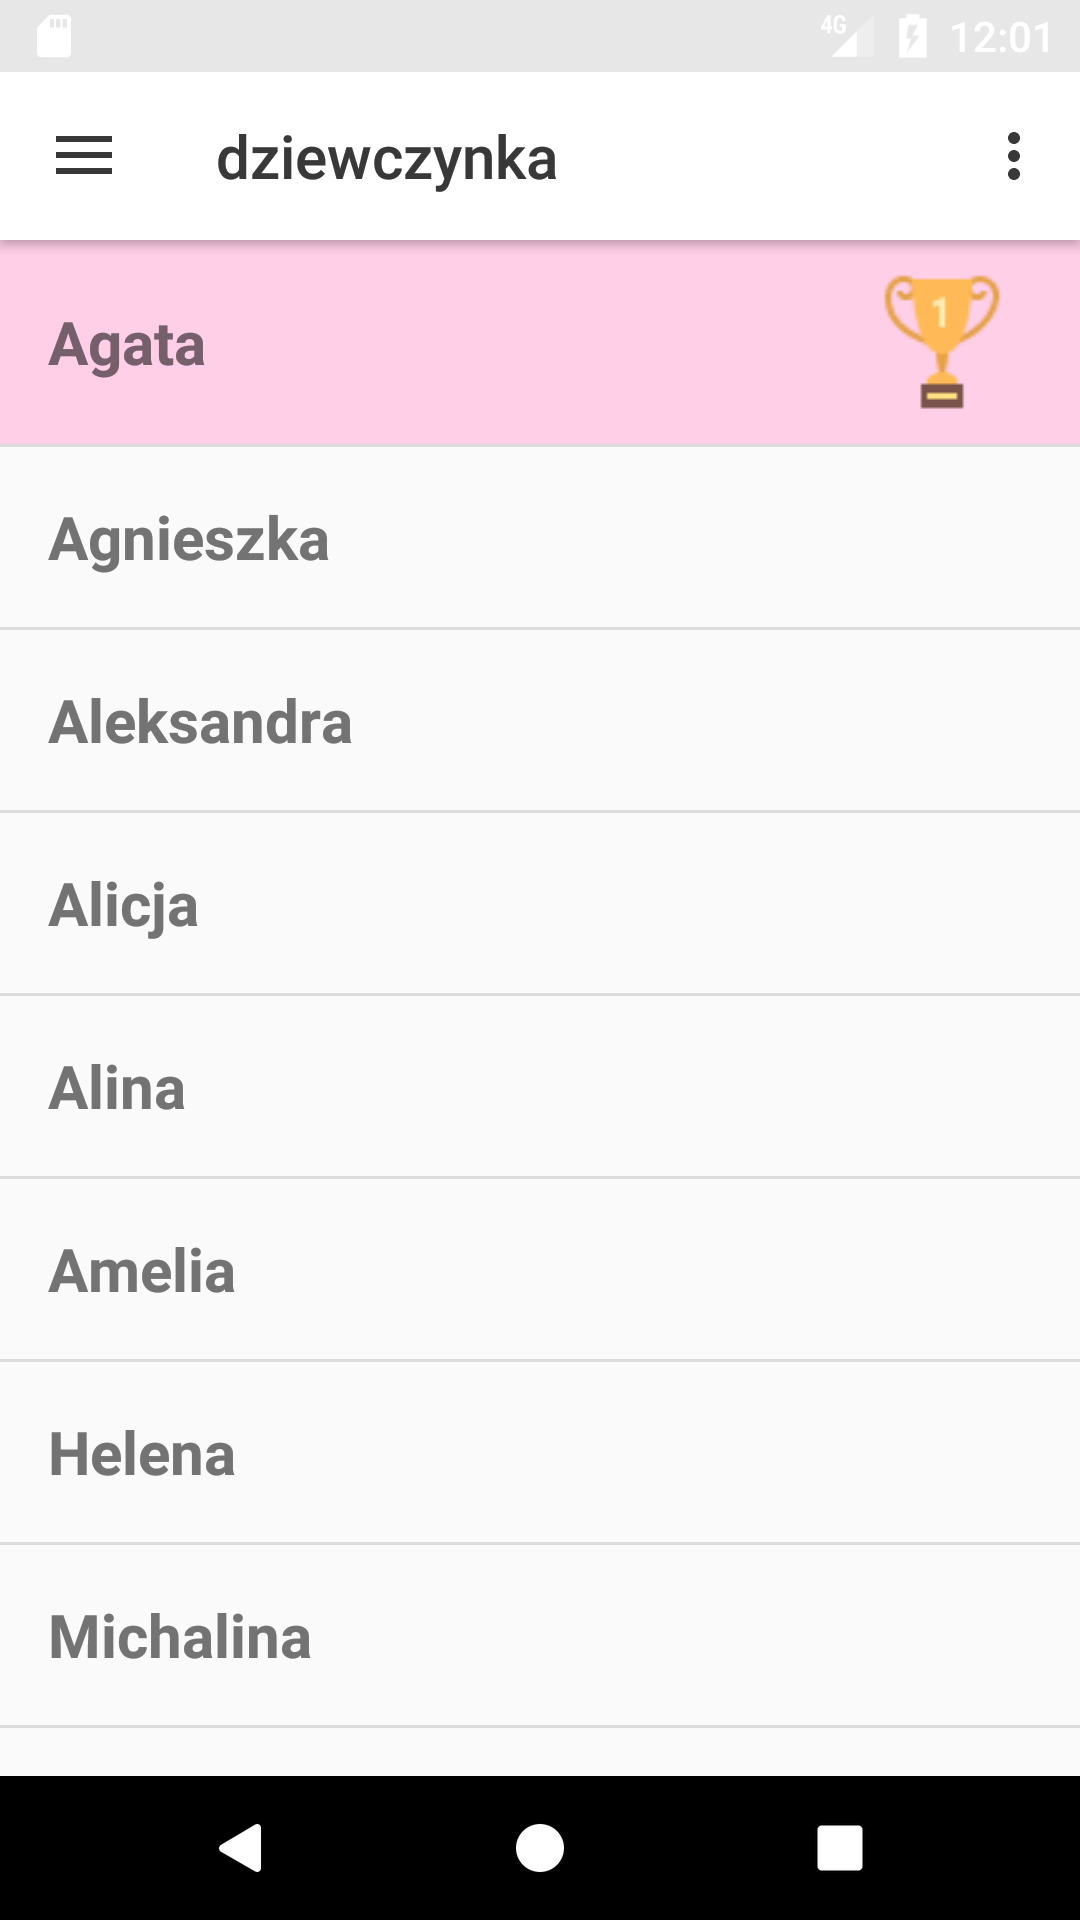
\includegraphics[width=0.5\textwidth]{top}
\end{figure}

\subsection{Opisy imion}
Niektórzy użytkownicy przywiązują dużą wagę do znaczenia imienia.
Dlatego udostępniamy możliwość przeczytania opisu wybranych imion.

\begin{figure}[h]
    \caption{Widok opisu imienia}
    \centering
    
\includegraphics[width=0.5\textwidth]{name_description}
\end{figure}

\section{Opis rozwiązania}
\subsection{Wstęp}

W projekcie można wyróżnić dwie zasadnicze części: klient (jako aplikacja na system Android) oraz serwer (wystawiający API -- poprzez HTTPS -- skrypt pythonowy).
Jako systemu kontroli wersji użyliśmy narzędzia Git.
Koordynację działań zespołu wspomagał GitHub, na którym umieściliśmy 3 repozytoria: dla kodu klienta, serwera oraz tekstu raportu.

\subsection{Klient}
Naturalnym wyborem do stworzenia klienta był język Java.
Cały zespół wykorzystywał Android Studio jako główne IDE.
Do testów użyty został framework JUnit.

Ze względu na komunikację klienta z serwerem, przydatne okazały się biblioteki Retrofit oraz gson.
W zestawieniu umożliwiają one wygodną realizację mapowania odpowiednich \textit{restfulowych} odpowiedzi na \textit{javowe} obiekty (i na odwrót).

Klient używa bazy danych SQLite do przechowywania informacji dot. utworzonych rankingów, loginu i hasła użytkownika, a także bazy imion.

\subsection{Serwer}
Część serwerowa została napisana przy użyciu języka Python 3 oraz frameworku Flask, który służy do tworzenia aplikacji webowych.
API umożliwia następujące akcje:

\begin{itemize}
    \item Utworzenie konta użytkownika;
    \item Utworzenie rankingu;
    \item Dodanie oceny danej pary imion;
    \item Pobranie listy par do ocenienia;
    \item Pobranie globalnego rankingu;
    \item Pobranie aktualnej bazy imion (wraz z opisami).
\end{itemize}

API jest udostępnione poprzez HTTPS.
Obsługę zapytań (oraz certyfikatów TLS/SSL) zapewnia nginx, który w naszym projekcie pełni funkcję WWW oraz serwera proxy.
API do wymiany danych wykorzystuje format JSON.

Serwer wykorzystuje również bibliotekę SQLAlchemy, która jest popularnym pythonowym ORM-em.
Umożliwa to stosunkową łatwą zmianę wykorzystywanej bazy danych w razie takiej potrzeby.
Do celów deweloperskich wykorzystywaliśmy bazę SQLite.

API jest dostępne pod adresem https://api.namefactory.pl.

\subsection{Ranking}
W celu stworzenia spersonalizowanego rankingu imion, wykorzystaliśmy tzw. ranking szachowy (elo).
Używany jest on zarówno przez klienta -- do budowania rankingów danego użytkownika -- jak i przez serwer -- do budowania rankingu globalnego.
Aktualnie używany jest w tej samej wersji, ale są to niezależne implementacje, umożliwiające -- przykładowo -- zmianę sposobu liczenia rankingu globalnego bez wpływania na rankingi użytkowników.

Zastosowaliśmy ranking szachowy z domyślną wartością dla każdego imienia wynoszącą \(1200\), oraz ze współczynnikiem \(K\) równym \(64\).
Wysoki współczynnik \(K\) umożliwia szybkie zmiany w rankingu, kosztem jego stabilności.
Uznaliśmy to za stosowny kompromis, ponieważ imion jest wiele, a nie chcemy wymagać od użytkownika dużej liczby ocen, aby ranking przybrał postać bliską prawdy.

\end{document}

